\documentclass{article}

\usepackage{amsmath, amsthm, amssymb, amsfonts}
\usepackage{thmtools}
\usepackage{graphicx}
\usepackage{setspace}
\usepackage{geometry}
\usepackage{float}
\usepackage{hyperref}
\usepackage[utf8]{inputenc}
\usepackage[english]{babel}
\usepackage{framed}
\usepackage[dvipsnames]{xcolor}
\usepackage{tcolorbox}

\colorlet{LightGray}{White!90!Periwinkle}
\colorlet{LightOrange}{Orange!15}
\colorlet{LightGreen}{Green!15}

\newcommand{\HRule}[1]{\rule{\linewidth}{#1}}

\declaretheoremstyle[name=Theorem,]{thmsty}
\declaretheorem[style=thmsty,numberwithin=section]{theorem}
\tcolorboxenvironment{theorem}{colback=LightGray}

\declaretheoremstyle[name=Proposition,]{prosty}
\declaretheorem[style=prosty,numberlike=theorem]{proposition}
\tcolorboxenvironment{proposition}{colback=LightOrange}

\declaretheoremstyle[name=Principle,]{prcpsty}
\declaretheorem[style=prcpsty,numberlike=theorem]{principle}
\tcolorboxenvironment{principle}{colback=LightGreen}

\setstretch{1.2}
\geometry{
    textheight=9in,
    textwidth=5.5in,
    top=1in,
    headheight=12pt,
    headsep=25pt,
    footskip=30pt
}

% ------------------------------------------------------------------------------

\begin{document}

% ------------------------------------------------------------------------------
% Cover Page and ToC
% ------------------------------------------------------------------------------

\title{ \normalsize \textsc{}
		\\ [2.0cm]
		\HRule{1.5pt} \\
		\LARGE \textbf{\uppercase{Relatório do trabalho\\ Pet shop}
		\HRule{2.0pt} \\ [0.6cm] \LARGE{Ferramentas da Internet} \vspace*{10\baselineskip}}
		}
\date{}
\author{\textbf{Autores:} \\
		Clarice Cabrini\\
		Hillary Carla\\
            Lara Silva\\
            Maria Eduarda\\
            Sarah Luiza\\
		22/04/2025}

\maketitle
\newpage

% ------------------------------------------------------------------------------

\section{Introdução}
O Pet Shop oferece uma variedade de serviços. Dentre eles banho, tosa e consultas veterinárias,
sendo eles executados por funcionários especializados. Os clientes podem agendar os serviços
previamente ou por demanda. Cada um desses clientes pode possuir um ou mais animais de
estimação, porém cada animal possui apenas e obrigatoriamente um dono. As informações
armazenadas dos clientes são nome completo, CPF, e-mail, telefone, data de nascimento e
endereço completo. Cada animal possui código de cadastro, nome, espécie, raça, data de
nascimento, sexo e peso atual. O sistema registra dados sobre a saúde dos animais. Os serviços
oferecidos incluem banho, tosa, consulta, vacinação e aplicação de medicamento. Ele é
caracterizado por tipo, descrição, valor base, duração estimada e pode sofrer variação de preço
conforme o porte do animal. Os agendamentos dos serviços contém data e hora, status do
agendamento, animal a ser atendido, cliente e funcionário. Os funcionários são divididos em
diferentes cargos, como banhista, tosador, veterinário e atendente. Cada um deles possui código
de identificação, nome completo, telefone, e-mail, cargo e salário. Os veterinários fazem
consultas, aplicações de vacina e tratamentos diversos. Cada consulta é vinculada a um animal e
um veterinário e possui informações como data, relatório, diagnóstico e prescrição de
medicamentos. Cada veterinário possui uma ou mais especialidades. Além de serviço, o Pet
Shop realiza venda de produtos como rações, brinquedos, acessórios e medicamentos. Cada
produto possuem código, nome, descrição, preço, categoria e validade. Os produtos são
fornecidos por fornecedores que possuem identificação, razão social ou nome, telefone e CNPJ
ou CPF. Um fornecedor fornece vários produtos. Cada Compra é registrada por um código, data
da compra, valor total e lista de itens comprados, especificando valor e quantidade. Cada venda
pode envolver produtos ou serviços e é vinculada a um cliente. Ela é identificada por código,
data e hora, forma de pagamento, valor total e funcionário responsável pelo atendimento. O
sistema registra pagamentos, que podem ser realizados em dinheiro, cartão de crédito ou
débito, ou PIX, incluindo informações de parcelamento quando aplicável.

\newpage

\section{Descrição dos relacionamentos}

 1 - Executa (Funcionário – Serviço) 

Semântica: Relaciona os funcionários aos serviços que eles executam. 
Cardinalidade: Muitos-para-muitos (um funcionário pode executar vários serviços e um serviço pode ser executado por vários funcionários). 
Participação: Parcial para Funcionário (nem todo funcionário executa serviços). 
Participação: Total para Serviço (todo serviço deve ser executado por pelo menos um funcionário). 

2- Aplica (Veterinário – Vacina) 

Semântica: Relaciona os veterinários às vacinas que eles aplicam. 
Cardinalidade: Um-para-muitos (um veterinário pode aplicar várias vacinas, mas cada vacina é aplicada por apenas um veterinário). 
Participação: Parcial para Veterinário (nem todo veterinário aplica vacinas). 
Participação: Total para Vacina (toda vacina deve ser aplicada por um veterinário). 

3- Faz (Veterinário – Consulta) 

Semântica: Relaciona os veterinários às consultas que eles realizam. 
Cardinalidade: Um-para-muitos (um veterinário pode realizar várias consultas, mas cada consulta é feita por apenas um veterinário). 
Participação: Parcial para Veterinário (nem todo veterinário realiza consultas). 
Participação: Total para Consulta (toda consulta deve ser realizada por um veterinário). 

4- Agenda (Cliente – Serviço – Funcionário – Animal) 

Semântica: Relaciona clientes aos serviços agendados, envolvendo funcionário responsável e o animal atendido. 
Cardinalidade: Muitos-para-muitos (um cliente pode agendar vários serviços, um serviço pode ser agendado por vários clientes, envolvendo diferentes funcionários e animais). 
Participação: Parcial para Cliente (nem todo cliente agenda serviço). 
Participação: Total para Serviço (todo agendamento deve estar associado a um serviço). 

5- Participa (Animal – Consulta) 

Semântica: Relaciona os animais às consultas que participam. 
Cardinalidade: Muitos-para-muitos (um animal pode participar de várias consultas e uma consulta pode envolver vários animais). 
Participação: Parcial para Animal (nem todo animal passa por consulta). 
Participação: Total para Consulta (toda consulta deve estar vinculada a pelo menos um animal). 

6- Possui (Cliente – Animal) 

Semântica: Relaciona os clientes aos animais que possuem. 
Cardinalidade: Um-para-muitos (um cliente pode possuir vários animais, mas cada animal pertence a apenas um cliente). 
Participação: Parcial para Cliente (nem todo cliente possui animal). 
Participação: Total para Animal (todo animal deve estar associado a um cliente). 

7- Registra (Animal – Sistema) 

Semântica: Relaciona os animais ao sistema em que são registrados. 
Cardinalidade: Muitos-para-um (vários animais podem ser registrados em um único sistema). 
Participação: Total para Animal (todo animal deve estar registrado). 
Participação: Total para Sistema (todo sistema deve conter pelo menos um animal). 

8- Registra (Sistema – Pagamento) 

Semântica: Relaciona o sistema aos pagamentos registrados. 
Cardinalidade: Um-para-muitos (um sistema pode registrar vários pagamentos, mas cada pagamento é registrado em apenas um sistema). 
Participação: Total para Pagamento (todo pagamento precisa ser registrado). 
Participação: Total para Sistema (todo sistema deve registrar pagamentos). 

9- Registra (Sistema – Vendas) 

Semântica: Relaciona o sistema às vendas registradas. 
Cardinalidade: Um-para-muitos (um sistema pode registrar várias vendas, mas cada venda é registrada em apenas um sistema). 
Participação: Total para Venda (toda venda deve ser registrada em um sistema). 
Participação: Total para Sistema (todo sistema deve conter vendas registradas). 

10 - Realiza (Cliente – Compra) 

Semântica: Relaciona os clientes às compras que eles realizam. 
Cardinalidade: Um-para-muitos (um cliente pode realizar várias compras, mas cada compra é feita por apenas um cliente). 
Participação: Parcial para Cliente (nem todo cliente realiza compras). 
Participação: Total para Compra (toda compra deve estar vinculada a um cliente). 

11- Pertence (Compra – Produto) 

Semântica: Relaciona as compras aos produtos adquiridos. 
Cardinalidade: Muitos-para-muitos (uma compra pode ter vários produtos e um produto pode aparecer em várias compras). 
Participação: Total para Compra (toda compra deve conter produtos). 
Participação: Parcial para Produto (um produto pode não ter sido comprado ainda). 

12- Fornece (Fornecedor – Produto) 

Semântica: Relaciona os fornecedores aos produtos que eles fornecem. 
Cardinalidade: Um-para-muitos (um fornecedor pode fornecer vários produtos, mas cada produto pertence a apenas um fornecedor). 
Participação: Parcial para Fornecedor (nem todo fornecedor fornece produtos). 
Participação: Total para Produto (todo produto deve ser fornecido por um fornecedor). 


\begin{figure}

\section{Dicionário de Entidades}

    \centering
    \includegraphics[width=1\linewidth]{dicionario.petshop.2.pdf}
    \caption{Dicionário de entidades}
    \label{fig:placeholder}
\end{figure}

\begin{figure}
\section{Diagrama}
    \centering
    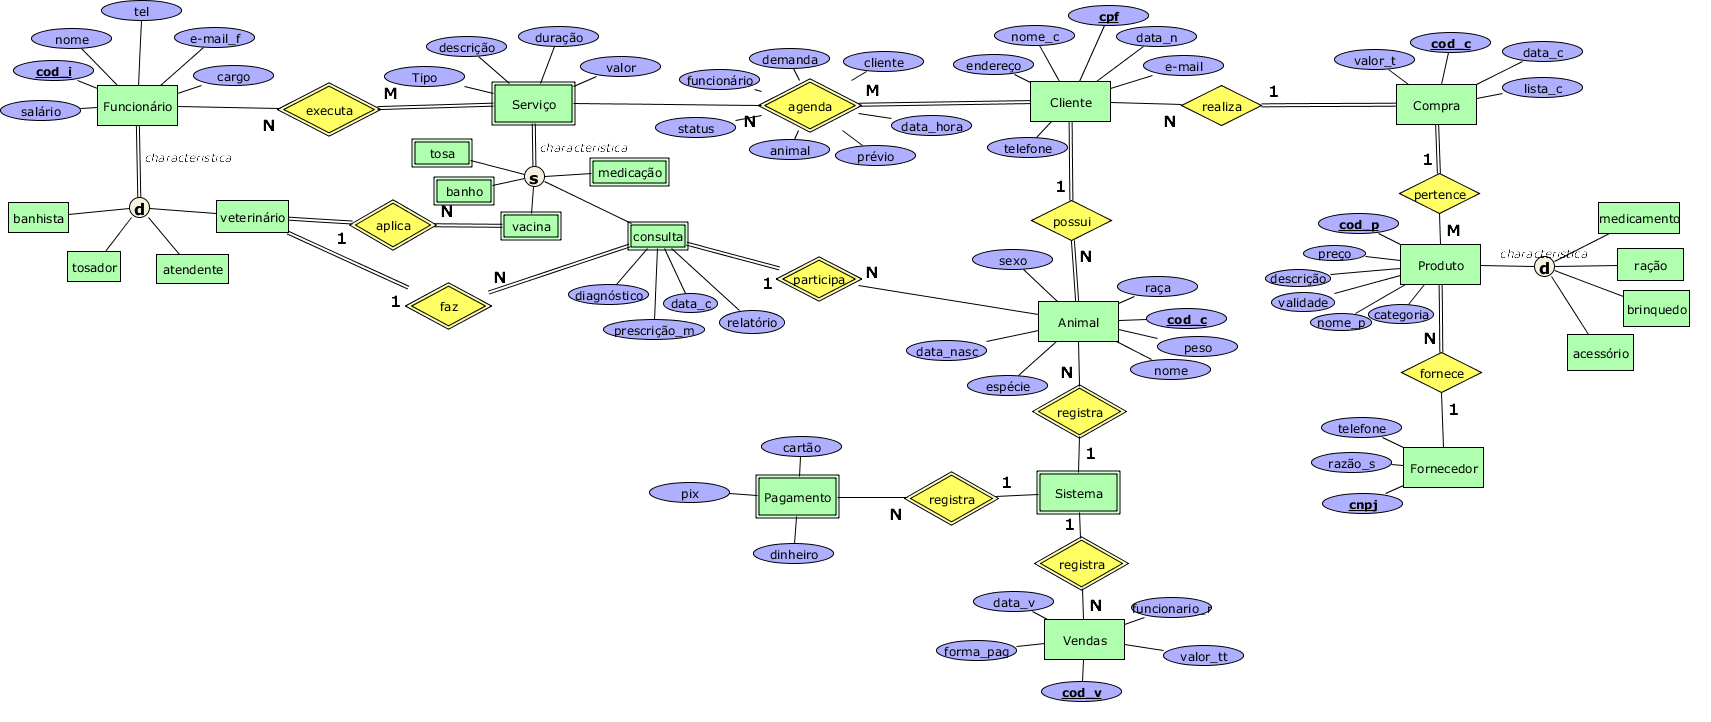
\includegraphics[width=1\linewidth]{diagrama.petshop.png}
    \caption{Figura - Diagrama Pet Shop}
    \label{fig:placeholder}
\end{figure}




\end{document}